%%%%%%%%%%%%%%%%%%%%%%%%%%%%%%%%%%%%%%%%%%%%%%%%%%%%%%%%%%%%%%%%%%%%%%%%%%%

\chapter{Vectors and Matrices}


%%%%%%%%%%%%%%%%%%%%%%%%%%%%%%%%%%%%%%%%%%%%%%%%%%%%%%%%%%%%%%%%%%%%%%%%%%%

\section{Scalars and vectors}
\label{sec:scalars_vectors}

The path of a car travelling from location $A$ to location $B$ is
characterized by two quantities or \emph{scalars}\index{scalars}: a
magnitude\index{magnitude}~(such as speed), and a direction~(from $A$
to $B$). Both of these two scalars are summarized by a
\emph{vector}\index{vector}.

\begin{figure}[!htpb]
\centering
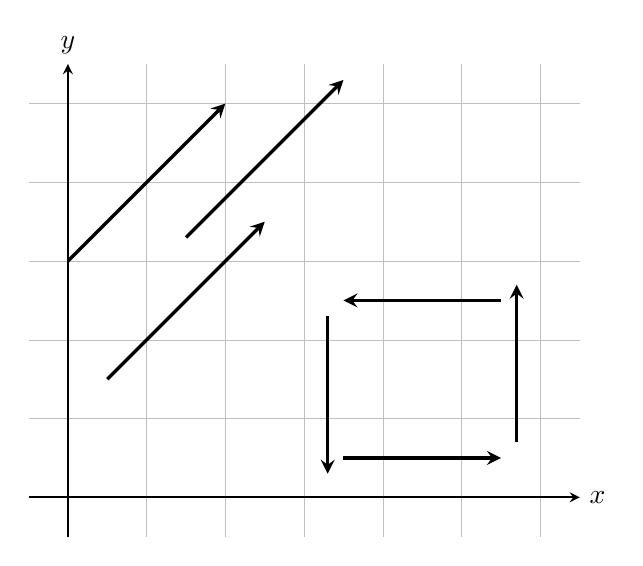
\begin{tikzpicture}
[linedecorate/.style={->,>=stealth,very thick}]
% grids for the plane
\draw[step=1cm,lightgray,very thin] (-0.5,-0.5) grid (6.5,5.5);
% the rectangular axes
\draw[->,>=stealth,semithick] (-0.5,0) -- (6.5,0) node[right]{$x$};
\draw[->,>=stealth,semithick] (0,-0.5) -- (0,5.5) node[above]{$y$};
% vectors
\draw[linedecorate] (0,3) -- node[above left]{$\vecu$} (2,5);
\draw[linedecorate] (1.5,3.3) -- node[below right]{$\vecv$} (3.5,5.3);
\draw[linedecorate] (0.5,1.5) -- node[below right]{$\vecw$} (2.5,3.5);
\draw[linedecorate] (3.5,0.5) -- (5.5,0.5);
\draw[linedecorate] (5.7,0.7) -- (5.7,2.7);
\draw[linedecorate] (5.5,2.5) -- (3.5,2.5);
\draw[linedecorate] (3.3,2.3) -- (3.3,0.3);
\end{tikzpicture}
\caption{Vectors in the $x$-$y$ plane.}
\label{fig:vectors_matrices:plane_vectors}
\end{figure}

In the $x$-$y$ plane, we can visualize a vector as an arrow from point
$A$ to point $B$~(see
Figure~\ref{fig:vectors_matrices:plane_vectors}). The starting point
$A$ of the vector is called the \emph{tail}\index{vectors!tail} and
the terminal point $B$ is the \emph{head}.\index{vectors!head} Two
vectors are \emph{equivalent}\index{vectors!equivalent} if they have
the same magnitude and direction. The vectors $\vecu$, $\vecv$, and
$\vecw$ in Figure~\ref{fig:vectors_matrices:plane_vectors} are thus
all equivalent to each other.

To analyze vectors using algebra, we can think of a vector $\vecu$
as starting from the origin of the $x$-$y$ plane and having
$(u_1, u_2)$ as the coordinate for its head~(see
Figure~\ref{fig:specify_vector_head_coordinate}). So $\vecu$ is
completely determined by the coordinate of its head and we write
$\vecu = \langle u_1, u_2 \rangle$ as an algebraic representation
for $\vecu$.

\begin{figure}[!htpb]
\centering
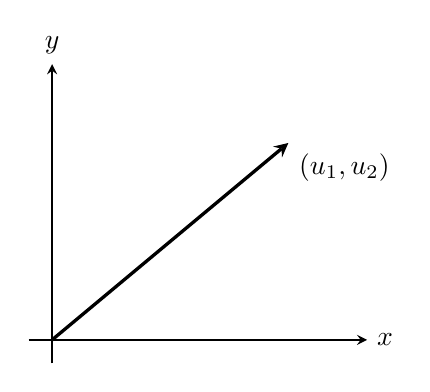
\begin{tikzpicture}
% the rectangular axes
\draw[->,>=stealth,semithick] (-0.3,0) -- (4,0) node[right]{$x$};
\draw[->,>=stealth,semithick] (0,-0.3) -- (0,3.5) node[above]{$y$};
% vector described by its head coordinate
\draw[->,>=stealth,very thick] (0,0) -- node[above left]{$\vecu$} (3,2.5) node[below right]{$(u_1, u_2)$};
\end{tikzpicture}
\caption{A vector as specified by its head coordinate.}
\label{fig:specify_vector_head_coordinate}
\end{figure}

In case the tail of $\vecu$ is not the origin, we let $(x_1, y_1)$
be the coordinate of the tail and denote the coordinate of the head by
$(x_2, y_2)$. By subtracting coordinatewise, we obtain an equivalent
vector $\vecv$ that emanates from the origin of the $x$-$y$
plane. The coordinate of $\vecv$ is
\[
(x_2, y_2) - (x_1, y_1)
=
(x_2 - x_1,\; y_2 - y_1)
=
(u_1, u_2)
\]
and we do not distinguish between $\vecu$ and $\vecv$. Thus we
can transform $\vecu$ to be a vector emanating from the origin and
specified by the coordinate
%
\begin{equation}
\label{eq:component_form_vector}
\vecu
=
\langle x_2 - x_1,\; y_2 - y_1 \rangle
=
\langle u_1, u_2 \rangle.
\end{equation}
%
Equation~(\ref{eq:component_form_vector}) is called the
\emph{component form}\index{component form} of a vector, with $u_1$
and $u_2$ being the individual components. The vector
$\veczero = \langle 0, 0 \rangle$ is called the zero
vector.\index{zero vector}

\begin{figure}[!htpb]
\centering
\begin{tikzpicture}
% the rectangular axes
\draw[->,>=stealth,semithick] (-2.5,0) -- (5.7,0) node[right]{$x$};
\draw[->,>=stealth,semithick] (0,-1.5) -- (0,6.7) node[above]{$y$};
% ticks on horizontal axis
\foreach \x in {-2,-1,-1}
  \draw (\x cm,2pt) -- (\x cm,-2pt) node[anchor=north] {$\x$};
\foreach \x in {1,2,...,5}
  \draw (\x cm,2pt) -- (\x cm,-2pt) node[anchor=north] {$\x$};
% ticks on vertical axis
\foreach \y in {-1,-1}
  \draw (2pt,\y cm) -- (-2pt,\y cm) node[anchor=east] {$\y$};
\foreach \y in {1,2,...,6}
  \draw (2pt,\y cm) -- (-2pt,\y cm) node[anchor=east] {$\y$};
% vector u
\draw[->,>=stealth,very thick] (-2,-1) node[below]{$(-2,-1)$} -- node[above left]{$\vecu$} (1,3) node[above]{$(1,3)$};
% vector v
\draw[->,>=stealth,very thick] (1.5,1.5) node[below]{$(1.5,1.5)$} -- node[above left]{$\vecv$} (4.5,5.5) node[above]{$(4.5,5.5)$};
\end{tikzpicture}
\caption{Verify that vectors $\vecu$ and $\vecv$ are equivalent.}
\label{fig:vectors_matrices:verify_vectors_u_v}
\end{figure}

\begin{example}
Let the vector $\vecu$ be described by the directed line segment
from $(-2,-1)$ to $(1,3)$, and let $\vecv$ be the line segment from
$(1.5,1.5)$ to $(4.5,5.5)$, as shown in
Figure~\ref{fig:vectors_matrices:verify_vectors_u_v}. Show that
$\vecu$ and $\vecv$ are equivalent vectors.
\end{example}

\begin{proof}[Solution]
To show that $\vecu$ and $\vecv$ are equivalent, we need to show
that they have the same length and are in the same direction. The
length of $\vecu$ is equivalent to the length of the line segment
from $(-2,-1)$ to $(1,3)$:
%
\begin{align*}
\sqrt{(1 - (-2))^2 + (3 - (-1))^2}
&=
\sqrt{(1 + 2)^2 + (3 + 1)^2} \\
&=
\sqrt{9 + 16} \\
&=
5.
\end{align*}
%
This tells us that $\vecu$ has length 5. Similarly, the length of
$\vecv$ is
%
\begin{align*}
\sqrt{(4.5 - 1.5)^2 + (5.5 - 1.5)^2}
&=
\sqrt{3^2 + 4^2} \\
&=
\sqrt{9 + 16} \\
&=
5
\end{align*}
%
which is the same length as that of $\vecu$.

\begin{lstlisting}
sage: u = vector([1 - (-2), 3 - (-1)]); u
(3, 4)
sage: v = vector([4.5 - 1.5, 5.5 - 1.5]); v
(3.000...000, 4.000...000)
sage: u.norm()
5
sage: v.norm()
5.000...000
\end{lstlisting}

The slope of the line segment from $(-2,-1)$ to $(1,3)$ is
\[
\frac{3 - (-1)} {1 - (-2)}
=
\frac{4}{3}
\]
and the slope of the line segment from $(1.5,1.5)$ to $(4.5,5.5)$ is
\[
\frac{5.5 - 1.5}{4.5 - 1.5}
=
\frac{4}{3}
\]
which shows that these two line segments have the same direction, so
$\vecu$ and $\vecv$ point in the same direction.
%
\begin{lstlisting}
sage: (3 - (-1)) / (1 - (-2))
4/3
sage: (5.5 - 1.5) / (4.5 - 1.5)
1.333...333
sage: QQ((5.5 - 1.5) / (4.5 - 1.5))
4/3
\end{lstlisting}
%
Therefore, $\vecu$ and $\vecv$ are equivalent vectors.
\end{proof}

We denote the length of a vector as follows. Let $\vecu$ be a
vector whose starting point is $P = (x_1, y_1)$ and whose terminal
point is $Q = (x_2, y_2)$. Then the length or magnitude of $\vecu$
is denoted by $\vecvertl \vecu \vecvertr$ and given
by the equation
%
\begin{equation}
\label{eq:vectors_matrices:magnitude_two_dimensional_vector}
\begin{aligned}
\vecvertl \vecu \vecvertr
&=
\sqrt{(x_2 - x_1)^2 + (y_2 - y_1)^2} \\
&=
\sqrt{v_1^2 + v_2^2}.
\end{aligned}
\end{equation}
